\chapter{INTRODUCCIÓN}


\section{Descripción General}

Desde los principios de la tecnología de semiconductores, los sistemas
electrónicos han venido experimentando un constante crecimiento en complejidad,
debido a que las prestaciones que tiene que ofrecer una aplicaciòn concreta son
cada vez mayores y de naturalezas màs diversas. Esto ha dado lugar a que un
sistema  tenga a la vez restricciones aparentemente incompatibles, como pueden
ser de trabajo en tiempo real, de tolerancia a fallos o de procesado de grandes
flujos de datos. Este incremento de complejidad y diversidad en las
restricciones ha motivado la apariciòn de diseños hìbridos en los que
interactùan elementos hardware y software, ya que dichos elementos pueden
complementarse para resolver problemas de distinta naturaleza.


Entre las alternativas para diseñar e implementar un hardware especìfico
encontramos ASICs  (Application-specific integrated circuit), FPGAs
(Field-programmable gate array), CPLDs (Complex Programmable Logic Device)
entre otros. El uso de ASICs posibilita desarrollos con producciòn a gran
escala a bajo costo y es de masiva utilizaciòn en este tipo de aplicaciones.
Los  CPLD  y las FPGA son circuitos de de alta densidad programables por el
usuario en un tiempo reducido y sin la necesidad de verificación de sus
componentes, tarea ya realizada por el fabricante al tratarse de un producto
estándar. El procesamiento digital de señales , prototipado de ASICs ,
tratamiento de imágenes , reconocimiento de voz , glue logic son algunas de las
aplicaciones de este tipo de dispositivos. Existen diferentes formas de llevar
adelante el diseño e implementación de un sistema digital para FPGA, entre
ellas tenemos la realización de un diseño esquemático , herramientas
específicas (provistas por el fabricante) y la utilización de un lenguaje de
descripción de hardware HDL (Hardware description language) entre los que  se
encuentran lenguajes como Verilog y VHDL, ambos de gran aceptación en los
ambientes industrial y académico. Estos lenguajes proporcionan gran
versatilidad para el desarrollo de hardware, permitiendo especificar, diseñar,
simular y verificar sistemas digitales complejos, mediante el apoyo de un
universo de herramientas EDA (Electronic Design Automation).

 Actualmente las FPGA cuentan con una gran cantidad de recursos disponibles
(Compuertas lógicas , Bloques de RAM) para implementar diseños digitales
complejos. Las FPGA pueden ser usadas para implementar cualquier función lógica
que un ASIC  pueda realizar. Una de las grandes ventajas del uso de FPGA en la
etapa de prototipado es su capacidad de reconfigurar el diseño parcial o
totalmente para su actualización o corrección de errores con un costo
relativamente bajo a diferencia del prototipado sobre ASICs. Durante la etapa
de producción los  ASIC resultan de muy bajo costo respecto de la producción de
FPGA y esto se traduce en una gran ventaja para desarrollos que deben ser
producidos a gran escala.

El desarrollo de aplicaciones de software se ve limitado a los recursos
disponibles en los microprocesadores comerciales. El software necesita del
soporte de un procesador para su ejecución, así la elección de este elemento
conlleva algunas dependencias respecto de las herramientas a utilizar , algunas
de estas son : compiladores , ensambladores , depuradores y herramientas de



\begin{figure}
\centerline{
        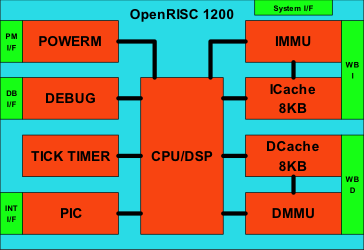
\includegraphics[width=12cm]{images/OR1200.png}
}
\caption{OpenRISC 1200 - Diagrama de Modulos}
\end{figure}

\section{Objetivos}
\subsection{Objetivo General}

Implementar un system on chip Open Source con un Softcore OpenRisc que soporte Linux, con la finalidad de entregar un  sitema integral FPGA-SoC-Sistema Operativo completamente funcional.

\subsection{Objetivo Especìfico}
\begin{itemize}
\item Evaluar, seleccionar y validar las prestaciones de los Kit de desarrollos con FPGA disponibles en el área de trabajo.
\item Obtener un System on Chip completamente funcional sobre un kit de desarrollo XILINX XtremeDSP Starter Platform Spartan 3A DSP 1800.
\item Implementar un Sistema Operativo en el Kit de desarrollo XILINX XtremeDSP Starter Platform Spartan 3A DSP 1800.
\item Probar el adecuado funcionamiento de el sistema global que tenga las  prestaciones funcional  
tradicionales de diseño
\end{itemize}

\section{Motivación} 

Desde el comienzo de la tecnología de semiconductores, los sistemas electrónicos han experimentando un constante crecimiento en complejidad, en consecuencia las prestaciones que tiene que ofrecer una aplicación concreta son cada vez mayores y de naturalezasmás diversas.
 Esto ha dado lugar a que un sistema tenga a la vez restricciones aparentemente incompatibles, como pueden ser de trabajo en tiempo real, de tolerancia a fallos o de procesado de grandes flujos de datos. 
Este incremento de complejidad y diversidad en las restricciones ha motivado  al desarrollo de diseños híbridos en los que interactúan elementos hardware y software, dichos elementos pueden complementarse para resolver problemas de distinta naturaleza.

Entre las alternativas para diseñar e implementar un hardware específico se encuentran FPGAs (Fieldprogrammable gate array) circuitos de alta densidad programables por el usuario en un tiempo reducido y sin la necesidad de verificación de sus componentes, tarea ya realizada por el fabricante al tratarse de un producto estándar.

Los lenguajes que se utilizan para diseñar e implementar un sistema digital sobre una FPGA proporcionan gran versatilidad para el desarrollo de hardware, permitiendo especificar, diseñar, simular y verificar sistemas digitales complejos, mediante el apoyo de un universo de herramientas EDA (Electronic Design Automation)
Las arquitecturas reconfigurables de las FPGA combinan parte de la flexibilidad del software con la gran performace del hardware.

Los  a veces requieren nuevas características de los cores existentes.El proveedor del núcleo puede hacer estas modificaciones (solución comercial) con un incremento sustancial del coste del núcleo. Otra posibilidad (Solución Ad-hoc) es el uso de cores de código abierto con el fin de crear un núcleo de desarrollo adaptable. El enfoque de código abierto tiene varias ventajas: el núcleo posee un costo muy bajo e inclusive cero, los usuarios puede tener acceso al código fuente y hay un grupo de desarrolladores que proporcionan conocimientos para mantener y mejorar el núcleo.

Los microprocesadores “softcore"(núcleo software) son aquellos cuyo hardware está íntegramente implementado en un lenguaje de descripción de hardware.Posibilitan un desarrollo confiable con facilidad de ajustar el mismo a las necesidades de aplicación que deben satisfacerse e incluso el desarrollo de microprocesadores doble o múltiple núcleo.
Entre los microprocesadores softcore encontramos los Open Source (Código Abierto) uno de ellos OpenRISC de Open Cores.
El procesador OpenRISC de 32 bits se comunica con sus periféricos por medio de un bus tipo Wishbone , también de código abierto. OpenRISC puede ser implementado
fácilmente en chips de cualquier fabricante (Xilinx , Altera , Actel) razón por la cual es el elemento central de algunos proyectos SoC de código abierto como MinSoC y 
de OpenCores u ORPSoC de OpenCores. 
Toda la implementación del proyecto posee una licencia LGPL lo que otorga al programador la capacidad de modificar el código a necesidad. Un conjunto de herramientas de desarrollo de software (compilador, ensamblador, debugger) también de código abierto ayudan al desarrollo de aplicaciones para esta arquitectura y son provistas en el proyecto OpenRISC.

Si bien la placa seleccionada, ZedBoard, soporta tanto Android como GNU/Linux nos motivó utilizar este último por lo siguiente:
Es el SO que por defecto viene instalado en la placa
Es un SO abierto con vasta documentación detallada y una gran comunidad.
La mayoría de los proyectos documentados con la utilización de esta placa han sido con GNU/Linux.
Todas las guías provistas por el fabricante se basan en este SO.

Que el sistema operativo sea multitarea.
2
Que el sistema operativo disponga de mecanismos de sincronización. 3 Que el sistema operativo soporte arquitecturas de sistemas embebidos.
Por todo esto, y puesto que se cumplen los requerimientos enunciados en al apartado 8.2, es que decidimos desarrollar este proyecto sobre GNU/Linux.

\section{Metodologìa}



\section{Importancia del Problema}

El softcore OpenRisc  que se encuentra en el SoC OrpSoc y MinSoc se tiene que implementado en una Spartan 3A de Xilinx. Tenemos como fin montar un Linux para validar y verificar el sistema global entregando un sistema funcional bajo licencia libre.
Actualmente las FPGAs nos birndan la posibilidad de implementar estos proyectos, donde el Hardware y el Software son una misma entidad. Este nuevo enfoque nos permite aprovechar la facilidad de implementar soluciones por Hardware.

\section{Alcance de Estudio}
\section{Modelo de Desarollo}
\section{Metodologìa}



 \section{Organización del Proyecto Integrador}

 Una vez detalladas  las motivaciones y expuestas las  ventajas que un
 receptor  coherente puede  aportar a  las comunicaciones  ópticas, el
 presente proyecto tiene como  principal objetivo el estudio, diseño y
 la simulación de los  diferentes métodos de recuperación de portadora
 de un receptor digital coherente para lo cual se organiza
 su contenido de la siguiente manera:\\

%%%%% poner en negrita asi \textit{Python} 


